\documentclass[10pt,final,journal]{IEEEtran}
\usepackage{xcolor} % Allows to make use and define many colors.
\usepackage[numbers]{natbib}
\usepackage{graphicx}
\usepackage{hyperref} 


%flowchart DOT code
%digraph G {
%	rankdir=LR
%	node [shape = rectangle]
	
%	a[label="Input video"]
%	b[label="Painting segmentation\n with bounding box"]
%	c[label="Painting transformation\n to standard format"]
%	d[label="Feature detection\n using brute force\n ORB matcher"]
%	e[label="Comparing feature vector\n against other paintings in dataset"]
%	f[label="Plot location of painting on ground plan"]
%	
%	a -> b [label="frames"]
%	b -> c [label="segmented painting"]
%	c -> d [label="painting in\n standard format"]
%	d -> e [label="feature vector"]
%	e -> f [label="match result"]
%	
%	{rank=same; a d}
%	{rank=same; b e}
%	{rank=same; c f}
%}


\newcommand{\todo}[1]{\color{red}\_ToDo: #1 \color{black}}
\graphicspath{{./img/}}
\title{Continuous room localization using painting detection}
\author{Bert De Saffel, Timothy Thiecke}
\begin{document}
	\maketitle
	\begin{abstract}
		This paper describes a localisation method based on paintings from a museum, in this particular case The Museum of Fine Arts, Ghent. The method consists of three parts. The first part is painting segmentation which attempts to detect a painting from an arbitrary video frame using painting contours and a bounding box and transforms this painting into a standard format such that it can be used for analysis. The second part considers the transformed image and uses a brute-force ORB \cite{Rublee2011} matcher to detect key features and descriptors. These features are matched against a database using a linear lookup method. The third step uses the information of the painting, which contains the room it is located in, to mark it on a ground plan of the museum.

	\end{abstract}

	\input{./tex/Introduction.tex}
	\section{Painting Detection}
\label{sec:painting_detection}




	The core of this work is painting detection, which consists of two steps: painting segmentation and feature matching. The segmentation tries to extract paintings from an arbitrary image while feature matching attempts to find distinguishable features of the extracted paintings and to match it against a database of paintings.

	\subsection{Painting Segmentation}
	The first step of the algorithm is the segmentation of an arbitrary video frame to detect a painting. A typical painting contains the art on its own enclosed by a painting frame. This painting frame causes a strong change in environment around its edges. For that reason, the Canny operator is applied to the initial video frame, resulting in a new image which contains strong edges. Afterwards, we attempt to find contours which yields a vector of points for each contour. To make this process easier and more accurate, a dilation step is first applied on the edge image. We consider only contours which consists of 4 points and take the first 10 which have the highest area, as paintings tend to have a higher area than other quadrilaterals on a video frame. It is possible that multiple paintings exist on a single video frame. However, the algorithm's goal is to detect in which room the user is located, and not in particular which painting it is. Multiple paintings on the same wall belong to the same room. If the painting segmentation step selects either one of these paintings, the end result will be the same. 
	

	The detected painting is then transformed through a homography to a rectified version which serves as the input of the following stage, feature detection and matching.

	\subsection{Feature Detection and Matching}
	Feature detection and extraction is applied to the extracted painting from the segmentation phase and will be matched with an image from the database. The detection of key features and descriptors is handled by ORB. Matching is done by invoking a matching procedure between the extracted keypoints and the keypoints of the database images. A match between descriptors is defined by its distance metric. The lower this number, the more likely that the match is valid. We calculate the sum of all matches and sort the matches between the source and database images by this sum. The first entry in this collection of matches is the image that is estimated to be a match for what is currently seen on-screen. 

	Additional meta-data is associated with the matched image and is used for the next phase.

	\subsection{Path Tracking}
	Once a painting is identified and matched, it can be localized on the ground plan. To achieve this, the ground plan is converted into a directed graph. The nodes of this graph are the rooms of the museum and the edges define the connections between rooms. When a painting is matched, its room is also known. This room can be marked on the graph in three distinct ways. A green node is the start of the path, an orange node is an intermediate path and the blue node is the end of the path. The path ends when the runtime loop ends. The path direction is also visualized by coloring the corresponding edges green. Note that when a cyclic path occurs which was walked in both directions, information of order of the nodes in this cycle is lost.


	To illustrate the path tracking algorithm,  a small segment consisting of rooms 1, 2, 3, 4, 5, 6, 7 and 8 are converted into such a graph and are show on figure \ref{fig:groundplan_msk_simple_graph}.


	%digraph G {
	%	2[fontcolor=white, fillcolor=green, style=filled]	
	%	4[fillcolor=orange, style=filled]
	%	5[fillcolor=orange, style=filled]
	%	7[fillcolor=orange, style=filled]
	%	6[fontcolor=white,fillcolor=blue, style=filled]
	%	1 -> 2
	%	2 -> 1
	%	2 -> 3
	%	2 -> 4[color=green]
	%	2 -> 5
	%	3 -> 2
	%	4 -> 2
	%	4 -> 5[color=green]
	%	4 -> 7
	%	4 -> 8
	%	5 -> 7[color=green]
	%	7 -> 6[color=green]
	%	6 -> 7
	%	7 -> 8
	%	7 -> 5
	%	7 -> 4
	%}

	\begin{figure}
		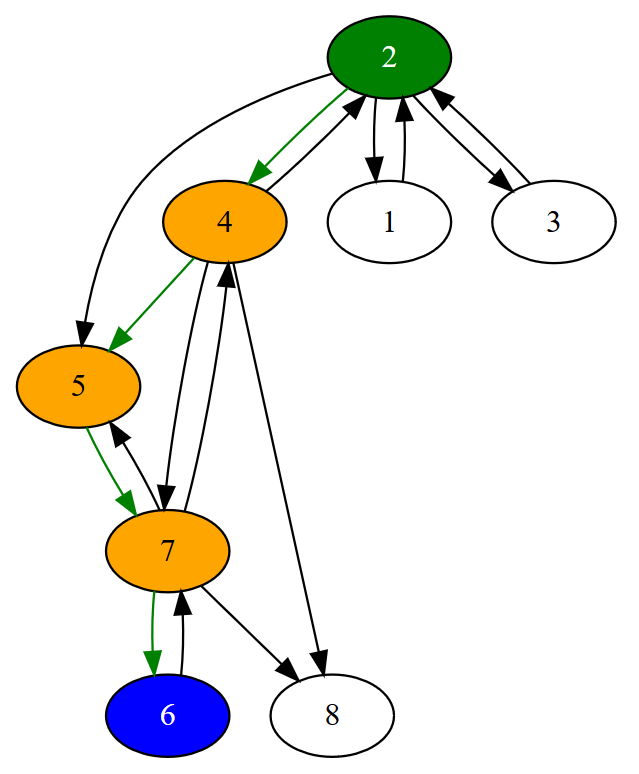
\includegraphics[width=\linewidth]{groundplan_msk_simple_graph}
		\caption{Path tracking using a graph. A green node marks the path's start, orange nodes the visited rooms, and blue the last node that was visited. Edges in green help visualize the path and the order which it was travelled.}
		\label{fig:groundplan_msk_simple_graph}
	\end{figure}


	
	\section{Results}
	Painting segmentation: 88.57 \% correct segmentation
	\todo{qualitative as well as quantitative}
	
	\todo{quantitative: graphs, tables, roc-curves, f1-scores, ...}
	
	\todo{qualititative: technisch, show where and why the method succeeds or fails, pictures of easy and difficulty cases}
	
	Because our method relies heavily on edge detection, there are cases where this could have a negative impact. In many cases, there is a shadow underneath the painting, as shown on figure \ref{fig:negative_case_shadow}.
	
	\begin{figure}
		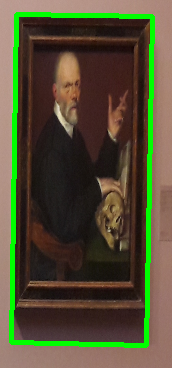
\includegraphics[width=\linewidth]{negative_case_shadow}
		\caption{An example of a shadow underneath the painting. This usually results in the segmentation algortihm to include this shadow as part of the painting because of the strong edge.}
		\label{fig:negative_case_shadow}
	\end{figure}

	\todo{stukje hierboven ook kwalitatief?}

\subsection{Qualitative analysis}
In this subsection, we will present a qualitative analysis of our algorithm. We will discuss its strengths, flaws and, with each point, present an example case to help as a visual aid. The flaws in particular help paint a picture of what can be done better in a future iteration of the algorithm. 


One of the algorithm's major strengths lies in its simplicity. The block diagram shows a very linear approach to the problem with concrete begin- and endpoints. Though machine learning is often used in the field of computer vision and has a lot of benefits, the algorithm does not employ it. We do not deny its usefulness and believe that it may be beneficial to implement it in a future version of the algorithm \todo{waar nodig?, kan zijn dat ML gebruikt wordt bij matching}. Even though the algorithm's simplicity is presented as one of its strengths, it can also be considered as one of its weaknesses, much like a double edged sword.


Furthermore, the algorithm works relatively fast for matching and determining the location of a potential user using a single image. Table \todo{tbl} gives an overview of the average elapsed time when running the algorithm on a single image. 
\todo{chart met timing van algoritme voor 1 afbeelding}


In addition, the use of ORB causes the results of each program run to be invariant given the same input image, implying a deterministic nature. This is of course on the premise that certain parameters such as the Canny thresholds remain the same between runs. Figures \todo{fig} and \todo{fig} shows how two images have the same match and detected keypoints between two runs. However, due to not detecting different potential candidate matches between runs results in the algorithm never being able to present a different solution for the given image.


On top of that, the algorithm is resilient when it can not successfully segment an image. The default behaviour is trying to find a frame, extract it, and using it as the input of the matching stage of the algorithm. If no frame can be found, rather than ignoring the current video frame or image, we supply the entire thing to be matched. This may slow the matching stage down by a small margin but has the benefit of still being able to spit out a potential positive match. Figure \todo{fig} shows an example where an entire frame is supplied to the matching function, but still manages to find a correct match.


As was hinted in the previous point, supplying a full frame or image to the matching phase may slow things down. The input image's size definitely affects the time needed to complete in a negative way. Therefore, images used for the segmentation and matching phases are resized to between \verb|25%-50%| their original size. This may result in some loss of precision but should not affect the overall efficiency of the algorithm. Table \todo{tbl} shows that resizing an image from the query set to a quarter of its size quadratically decreases the amount of pixels needed to evaluate. The same resizing is applied to the building stage of the database.


Another problem arises due to an assumption in the matching stage. A match is determined by the smallest sum of distances calculated over the matches between two images. This assumption works well when the amount of matches is fixed between every match between the query image and the training set. ORB detects keypoints and associates descriptors up to a maximum of 200. But what if it can not detect a lot of keypoints, maybe even none? Figure \todo{fig} shows how paintings that have a relative 'flat' surface without discerning features (even to the naked eye) have trouble being matched to a picture in the data set. Suppose that the segmentation phase detects such a painting and supplies it to the matching phase. A cascade of erroneous matches and room localizations may occur. The inverse is also true, as having an entry in the data set with few keypoints can result in a painting with many keypoints being wrongfully matched with a 'flat' one.


The final major flaw that will be presented lies in the matching phase: matching a painting is done by doing a linear lookup in the database. For a single image this does not pose that much of a problem. The same can not be said when we expanded our algorithm to analyze the frames of a video. This slowdown is mitigated through two changes to the original algorithm. First, we run it only every 30 or so video frames which is equivalent to around 1 second in real life. Suppose the user is using their smart phone's camera, even when running, it will take some time to cross from one room to the other. Finally, the algorithm offloads the matching procedure to a multithreading environment, freeing the video code from freezing. But what causes this freezing in the first place? 


Considering there are 688 pictures in the database, coupled with the keypoints and descriptors that were extracted during the prebuilding phase, are matched with the descriptors of the segmented painting results in a total.

Furthermore, there is also no stop condition to the lookup.
This suggests that our matching code has $O(n^{2})$ behaviour.
which with a small amount of pictures is not a factor that we can simply leave. A possible solution to this problem may lie in other journals \todo{ref naar boek/conference over bag of words/large databases}. \todo{laatste paragraaf herschrijven} \todo{https://github.com/opencv/opencv/blob/master/doc/py_tutorials/py_feature2d/py_matcher/py_matcher.markdown}
		\section{Conclusion}
	\todo{overview of the most important contributions and the results, without introducing anything new}
	
	\todo{after the reader has read the paper, the reader can look at the contributions and results from a different viewpoint}
	
	\todo{statements can be made more explicit}
	
	\todo{eventueel future work}

	\bibliographystyle{IEEEtran}
	\bibliography{IEEEabrv,library}
\end{document}